%----------------------------------------------------------------------------------------
%    PACKAGES AND THEMES
%----------------------------------------------------------------------------------------

\documentclass[aspectratio=169,xcolor=dvipsnames]{beamer}
\usetheme{SimplePlus}





\usepackage{graphicx}                 % Einfügen von Bildern


\graphicspath{{../figures/Base_Case/}{../figures/Dynamic_MisSpec/}{../figures/NonLinear_DGP/}} %Ref figures outside Latex Directory


\usepackage{hyperref}
\usepackage{graphicx} % Allows including images
\usepackage{booktabs} % Allows the use of \toprule, \midrule and \bottomrule in tables
\usepackage{xcolor}
\usepackage[most]{tcolorbox}
\setbeamertemplate{caption}[numbered]
\usepackage{babel}[german]

\usepackage{booktabs}

\usepackage{mathtools}

\setbeamercovered{transparent=15} 



% Definiere eine eigene Umgebung für Beispiele ohne Titel
\newtcolorbox{myexample}{
    colback=green!10,   % Hintergrundfarbe (leichtes Grün)
    colframe=white,     % Kein sichtbarer Rahmen
    sharp corners,      % Keine abgerundeten Ecken
    boxrule=0pt         % Keine Rahmenlinie
}

%----------------------------------------------------------------------------------------
%    TITLE PAGE
%----------------------------------------------------------------------------------------

\title{Local Projections or VARs: \\ Evidence from Monte-Carlo Simulations}
\subtitle{Aaron Liebig \& Patrick Tenner}

\author{Superv.: Prof. Dr. Derya Uysal}

\institute
{
    SPS Seminar \\
    Summer Semester 26
}
\date{\today} % Date, can be changed to a custom date

%----------------------------------------------------------------------------------------
%    PRESENTATION SLIDES
%----------------------------------------------------------------------------------------

\begin{document}

\begin{frame}
    % Print the title page as the first slide
    \titlepage
\end{frame}

\begin{frame}{Motivation}
    \begin{itemize}
        \item VARs and Local Projection used for Impulse Response Analysis, think Unemployment and Interest Rate, Oil Prices and Inflation, ...
        \item finite sample comparison (VAR(p) vs. LP(p))
        \begin{enumerate}
            \item In finite samples, bias-variance puzzle 
            \item VARs more efficient, LPs more robust to misspecification 
        \end{enumerate}
        \item In Population both estimate the same Impulse Response
        \item Ludwig identity shows that equal lag comparison is inherently flawed 
    \end{itemize}

\begin{myexample}
    \textbf{(BL:)} Where does a fixed LP(4) sit on the VAR complexity frontier and does the conventional equal-lag ranking sruvive? \\
    \textbf{(EX:)} Does any genuine LP advantage emerge once misspecification is introduced?
\end{myexample}

\end{frame}


%-----------------------------------------------------------------------------------
\begin{frame}{Agenda}
    \tableofcontents
\end{frame}


%-----------------------------------------------------------------------------------

\section{Theory}


\begin{frame}{VARs}

\begin{equation}
    Y_t =\mathbf{\nu} + \mathbf{A} Y_{t-1} + U_t \xRightarrow[restr. K]{A1}  y_t = \mu + \sum_{\ell=0}^{\infty} \Psi_\ell\, u_{t-\ell},
\qquad \Psi_\ell := [\mathbf{A}^\ell]
\end{equation}

\textbf{Identification:} As $\sum_u = \mathbb{E}[u_tu_t'] \neq I_K$, Define $u_t=B\varepsilon_t$ where $\varepsilon_t \sim (0, I_k)$


\begin{equation}
    y_{t+h} = \mu + \sum_{\ell=0}^{\infty} \Theta_\ell\, \varepsilon_{t+h-\ell} \qquad 
    \label{eq:sma_forward}
\end{equation}

% Which 
% \begin{itemize}
%     \item are asymptotically normal and efficient (under homoskedasticity)
% \end{itemize}
Suffer from
\begin{itemize}
    \item LS bias compunds as horizon grows Kilian 1998 
    \item near-unit root behavior 
    \item misspecification through MA dynamics or lag order
\end{itemize}
\end{frame}

\begin{frame}{LPs}

    \begin{equation}
    y_{t+h} = \alpha_h + \beta_h\, s_t
            + \boldsymbol{\gamma}_h'\, \mathbf{x}_t
            + \xi_{t+h}^{(h)},
    \qquad h = 0, 1, \ldots, H,
    \label{eq:lp_shock}
\end{equation}
    
\end{frame}

\begin{frame}{Equivalence and Ludwig identity}


\end{frame}
%-----------------------------------------------------------------------------------

\section{Study Design}

\begin{frame}{DGPs}
        
\end{frame}

\begin{frame}{Method}
        
\end{frame}


%-----------------------------------------------------------------------------------

\section{Results}

\begin{frame}{Baseline Results - Complexity Frontier}

\begin{figure}
    \centering
    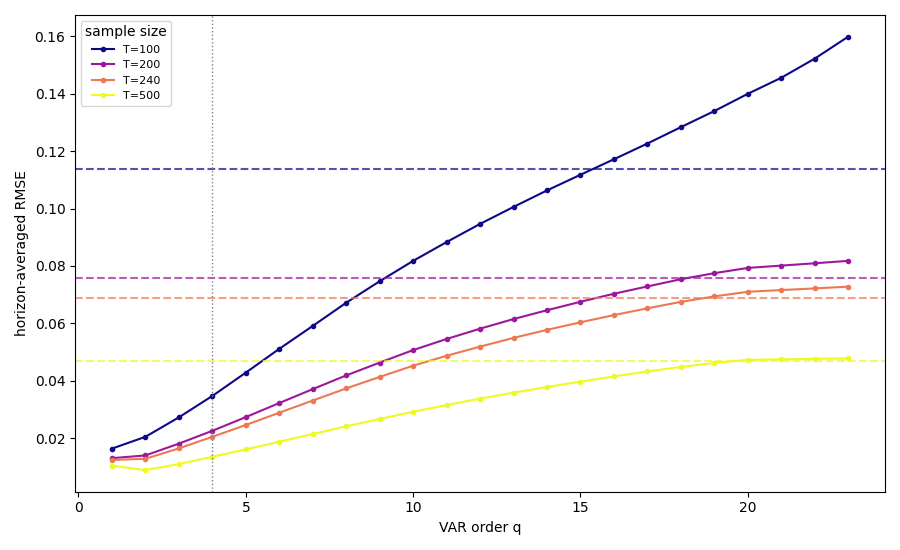
\includegraphics[width=0.7\linewidth]{BASE_COMPLEXITY_FRONTIER_rho=0.5.png}
    \vspace*{-0.2cm}
    \caption{Complexity Frontier $\rho = 0.5$}
\end{figure}
\end{frame}

\begin{frame}{Complexity Frontier - varying $\rho$} %1
    \begin{figure}
        \centering
        \begin{minipage}{0.59\textwidth}
            \centering
            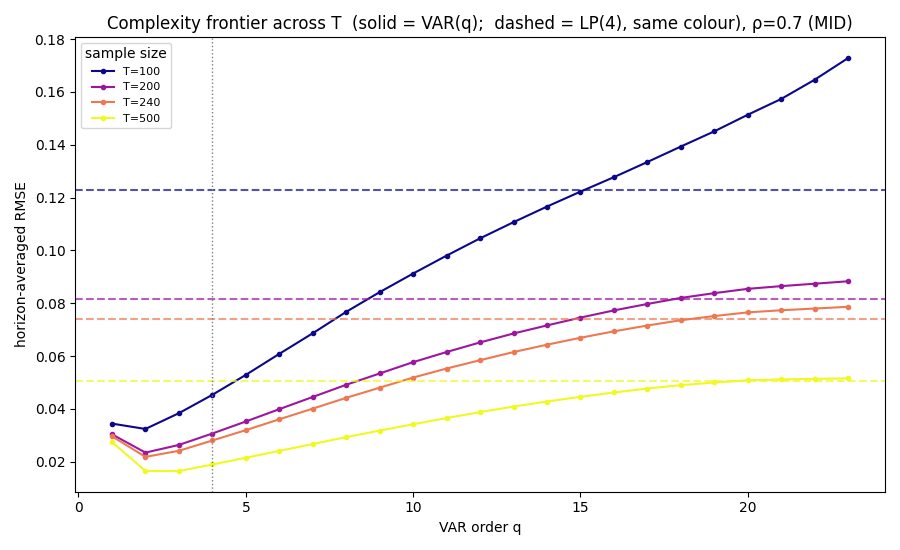
\includegraphics[width=\textwidth]{BASE_COMPLEXITY_FRONTIER_rho=0.7.png}
            \caption{Complexity Frontier $\rho = 0.7$}
        \end{minipage}
        \hfill
        \begin{minipage}{0.39\textwidth}
            \centering
            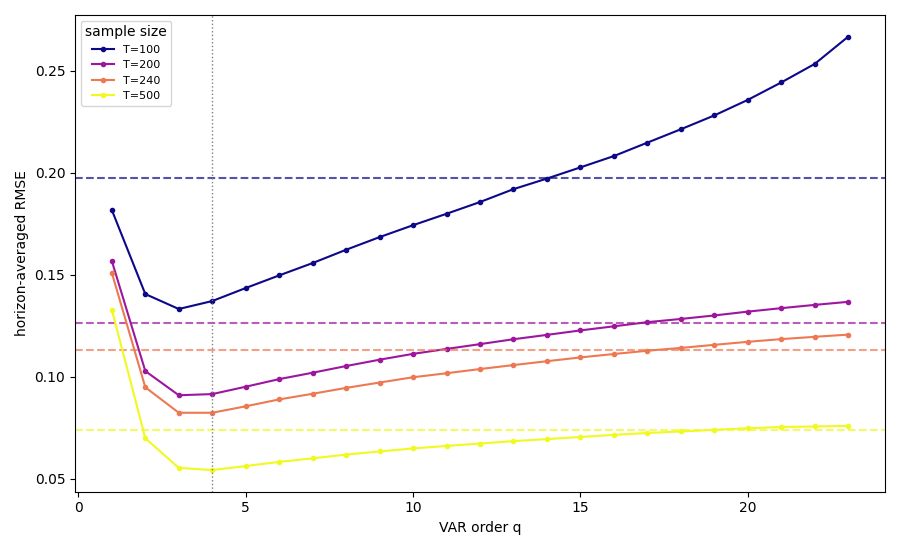
\includegraphics[width=0.8\textwidth]{BASE_COMPLEXITY_FRONTIER_rho=0.95.png}
            \caption{Complexity Frontier $\rho = 0.95$}
        \end{minipage}
    \end{figure}
\end{frame}

\begin{frame}[noframenumbering]{Complexity Frontier - varying $\rho$} %2
     \addtocounter{figure}{-2} 
    \begin{figure}
        \centering
        \begin{minipage}{0.39\textwidth}
            \centering
            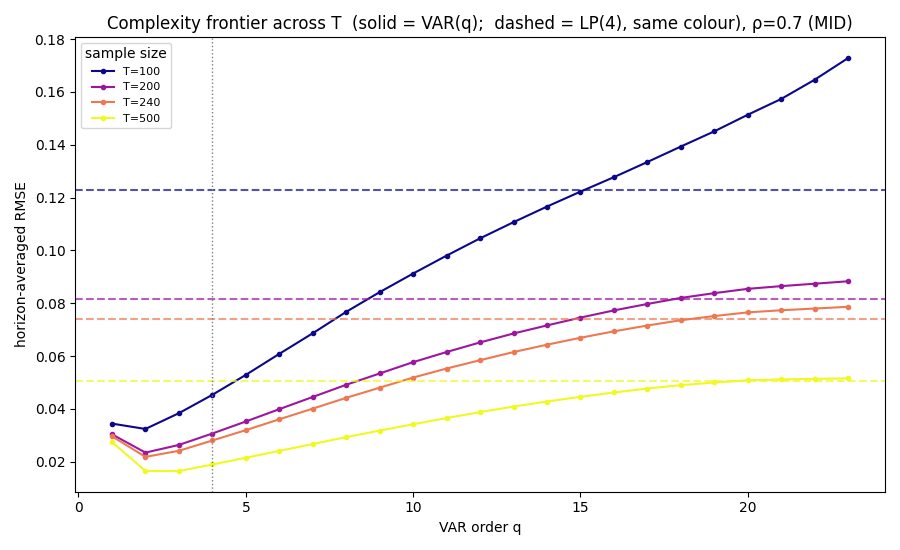
\includegraphics[width=0.8\textwidth]{BASE_COMPLEXITY_FRONTIER_rho=0.7.png}
            \caption{Complexity Frontier $\rho = 0.7$}
        \end{minipage}
        \hfill
        \begin{minipage}{0.59\textwidth}
            \centering
            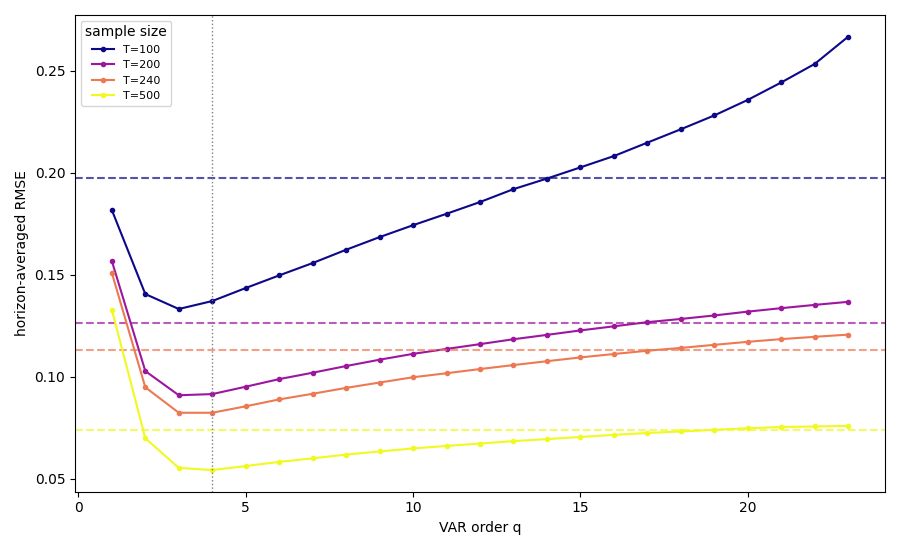
\includegraphics[width=\textwidth]{BASE_COMPLEXITY_FRONTIER_rho=0.95.png}
            \caption{Complexity Frontier $\rho = 0.95$}
        \end{minipage}
    \end{figure}
\end{frame}
%-----------------------------------------------------------------------------------

\begin{frame}{Bias}
    \begin{figure}
        \centering
        \begin{minipage}{0.59\textwidth}
            \centering
            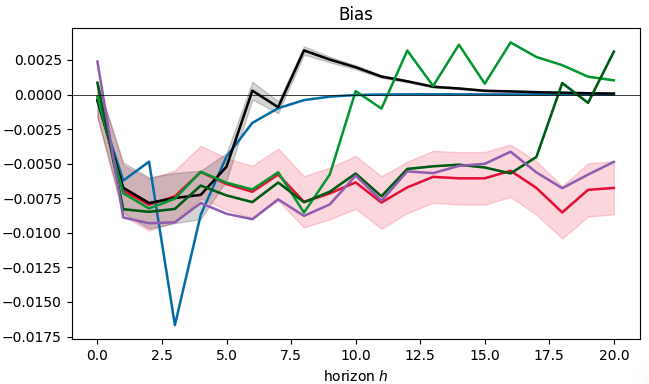
\includegraphics[width=\textwidth]{BASE_BIAS_0.5.png}
            \caption{Bias at $\rho = 0.5$}
        \end{minipage}
        \hfill
        \begin{minipage}{0.39\textwidth}
            \centering
            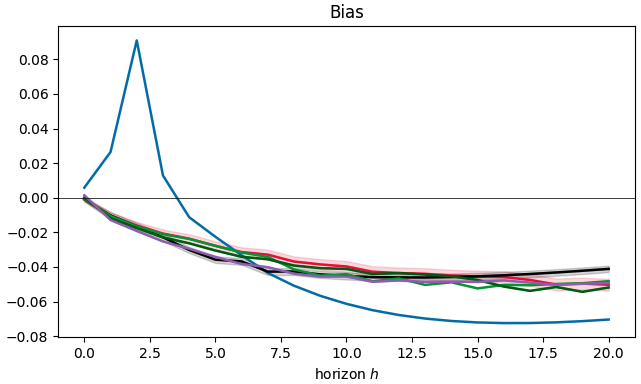
\includegraphics[width=\textwidth]{BASE_BIAS_0.95.png}
            \caption{Bias at $\rho = 0.95$}
        \end{minipage}
    \end{figure}
\end{frame}

\begin{frame}[noframenumbering]{Bias}
    \addtocounter{figure}{-2} 
    \begin{figure}
        \centering
        \begin{minipage}{0.39\textwidth}
            \centering
            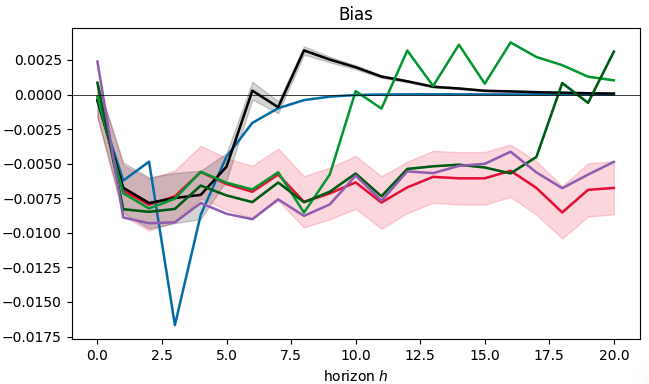
\includegraphics[width=\textwidth]{BASE_BIAS_0.5.png}
            \caption{Bias at $\rho = 0.5$}
        \end{minipage}
        \hfill
        \begin{minipage}{0.59\textwidth}
            \centering
            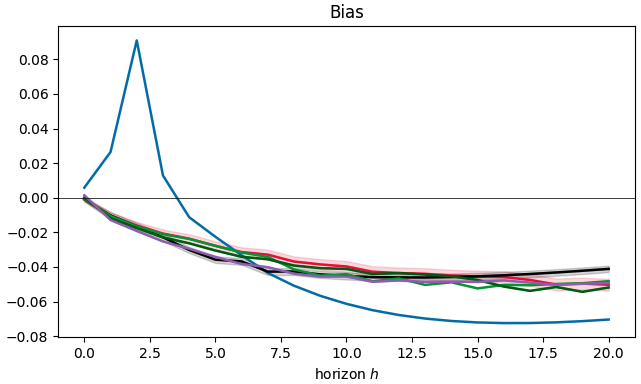
\includegraphics[width=\textwidth]{BASE_BIAS_0.95.png}
            \caption{Bias at $\rho = 0.95$}
        \end{minipage}
    \end{figure}
\end{frame}
%-----------------------------------------------------------------------------------

\begin{frame}{Variance}
    \begin{figure}
        \centering
        \begin{minipage}{0.59\textwidth}
            \centering
            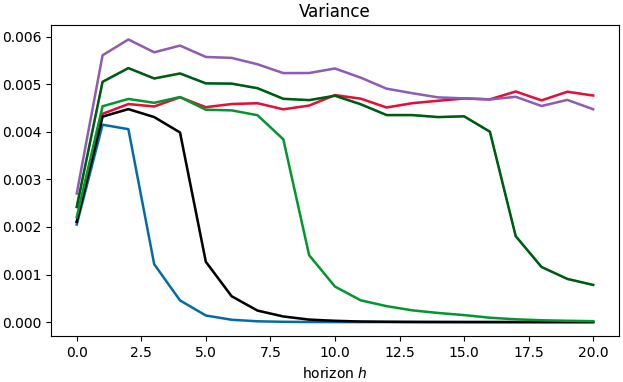
\includegraphics[width=\textwidth]{BASE_VAR_0.5.png}
            \caption{Variance at $\rho = 0.5$}
        \end{minipage}
        \hfill
        \begin{minipage}{0.39\textwidth}
            \centering
            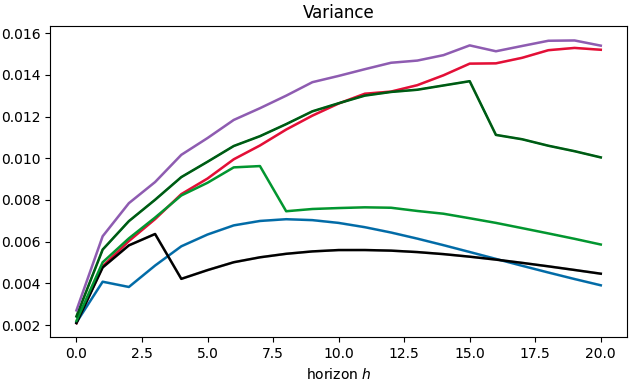
\includegraphics[width=\textwidth]{BASE_VAR_0.95.png}
            \caption{Variance at $\rho = 0.95$}
        \end{minipage}
    \end{figure}
\end{frame}

\begin{frame}[noframenumbering]{Variance}
    \addtocounter{figure}{-2} 
    \begin{figure}
        \centering
        \begin{minipage}{0.39\textwidth}
            \centering
            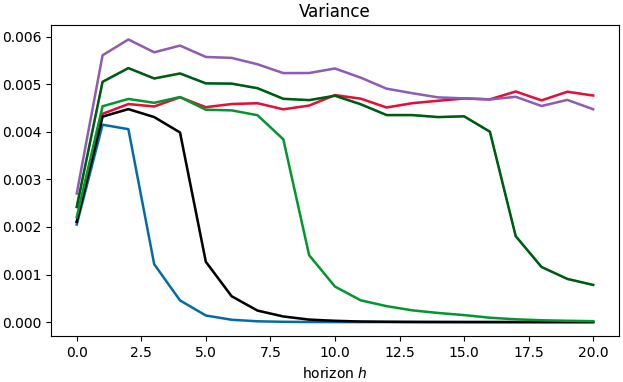
\includegraphics[width=\textwidth]{BASE_VAR_0.5.png}
            \caption{Variance at $\rho = 0.5$}
        \end{minipage}
        \hfill
        \begin{minipage}{0.59\textwidth}
            \centering
            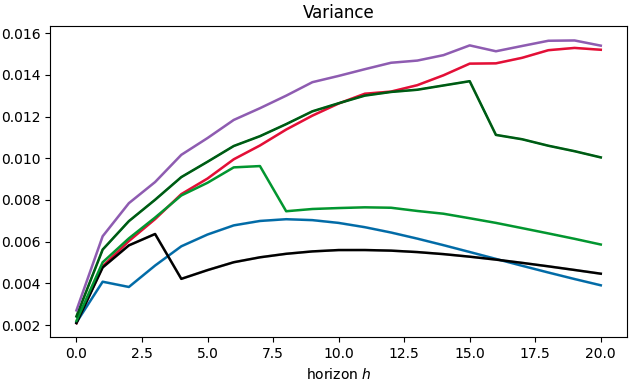
\includegraphics[width=\textwidth]{BASE_VAR_0.95.png}
            \caption{Variance at $\rho = 0.95$}
        \end{minipage}
    \end{figure}
\end{frame}
%-----------------------------------------------------------------------------------

\begin{frame}{Coverage}
    \begin{figure}
        \centering
        \begin{minipage}{0.59\textwidth}
            \centering
            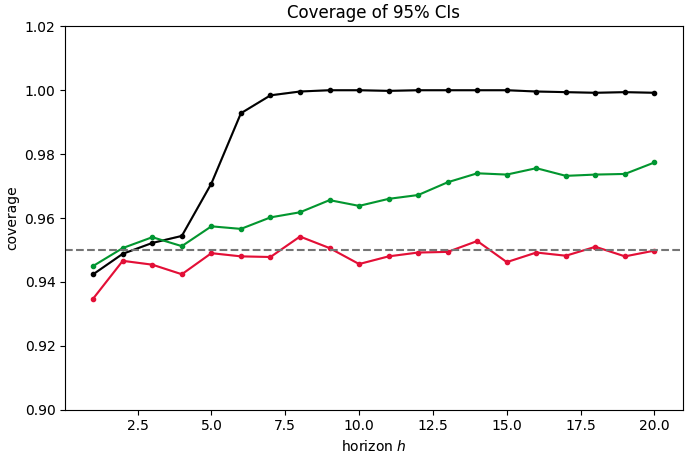
\includegraphics[width=\textwidth]{BASE_CI_0.5.png}
            \caption{Coverage at $\rho = 0.5$}
        \end{minipage}
        \hfill
        \begin{minipage}{0.39\textwidth}
            \centering
            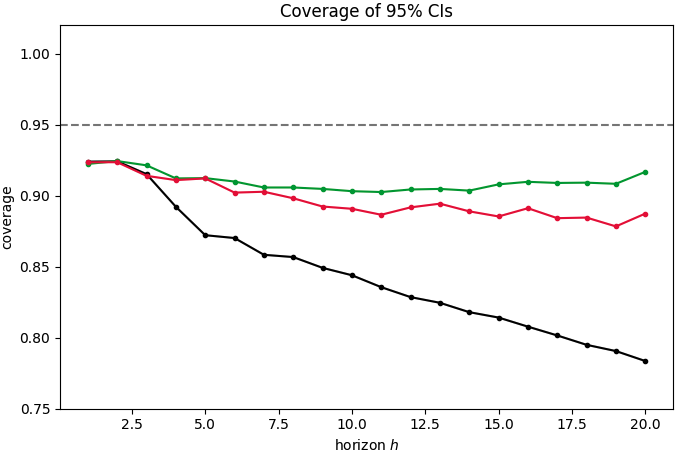
\includegraphics[width=\textwidth]{BASE_CI_0.95.png}
            \caption{Coverage at $\rho = 0.95$}
        \end{minipage}
    \end{figure}
\end{frame}

\begin{frame}[noframenumbering]{Coverage}
    \addtocounter{figure}{-2} 
    \begin{figure}
        \centering
        \begin{minipage}{0.39\textwidth}
            \centering
            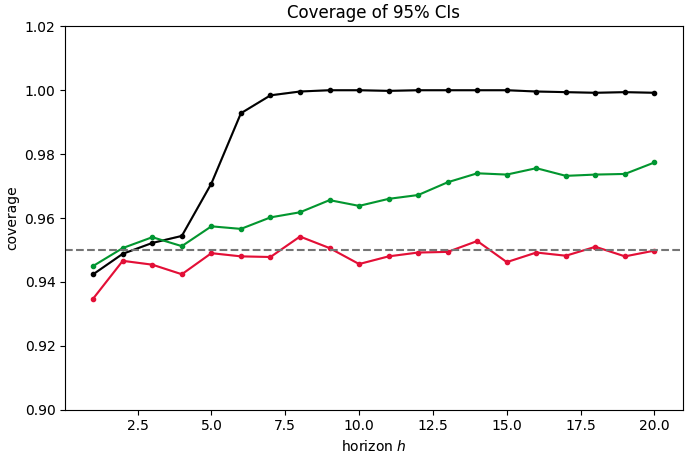
\includegraphics[width=\textwidth]{BASE_CI_0.5.png}
            \caption{Coverage at $\rho = 0.5$}
        \end{minipage}
        \hfill
        \begin{minipage}{0.59\textwidth}
            \centering
            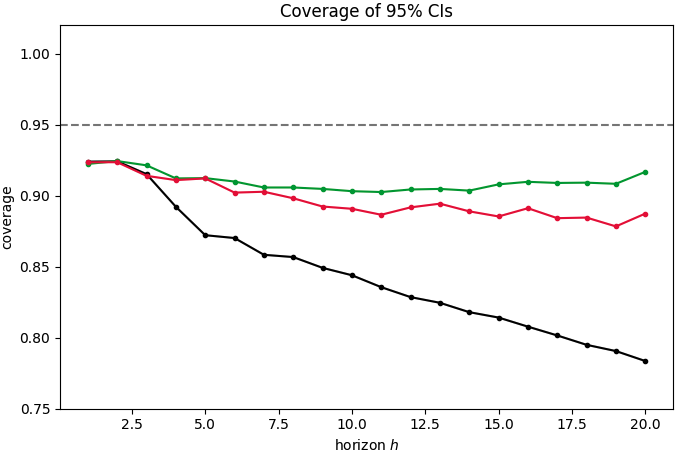
\includegraphics[width=\textwidth]{BASE_CI_0.95.png}
            \caption{Coverage at $\rho = 0.95$}
        \end{minipage}
    \end{figure}
\end{frame}


%------------------------------------------------
\begin{frame}{Introducing Dynamic Misspecification}

\begin{figure}
    \centering
    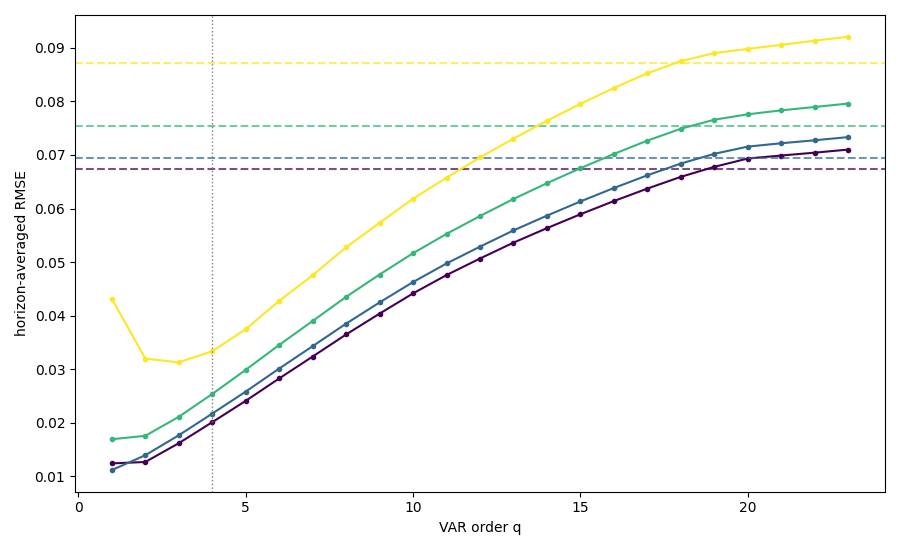
\includegraphics[width=0.7\linewidth]{DYN_MISSPEC_COMPLEXITY_FRONTIER_rho=0.5_T=250.png}
    \vspace*{-0.2cm}
    \caption{Complexity Frontier $\rho = 0.5$}
\end{figure}
\end{frame}

\begin{frame}{Dynamic Misspecification - varying $\rho$} %1
    \begin{figure}
        \centering
        \begin{minipage}{0.59\textwidth}
            \centering
            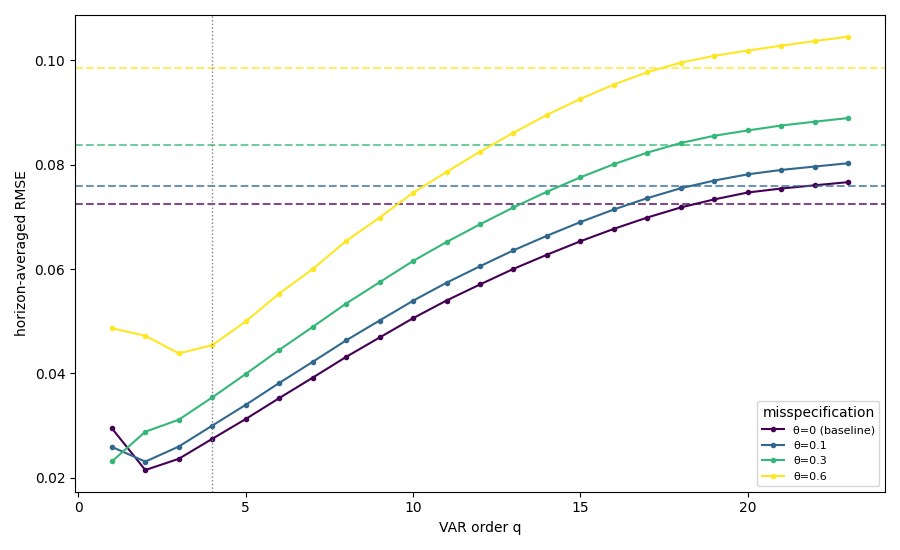
\includegraphics[width=\textwidth]{DYN_MISSPEC_COMPLEXITY_FRONTIER_rho=0.7_T=250.png}
            \caption{Complexity Frontier $\rho = 0.7$}
        \end{minipage}
        \hfill
        \begin{minipage}{0.39\textwidth}
            \centering
            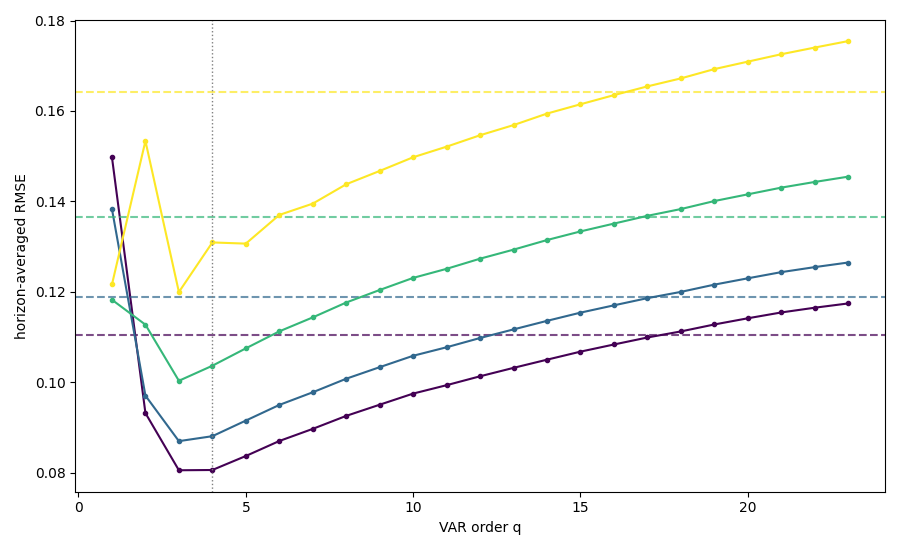
\includegraphics[width=\textwidth]{DYN_MISSPEC_COMPLEXITY_FRONTIER_rho=0.95_T=250.png}
            \caption{Complexity Frontier $\rho = 0.95$}
        \end{minipage}
    \end{figure}
\end{frame}

\begin{frame}[noframenumbering]{Dynamic Misspecification - varying $\rho$} %2
     \addtocounter{figure}{-2} 
    \begin{figure}
        \centering
        \begin{minipage}{0.39\textwidth}
            \centering
            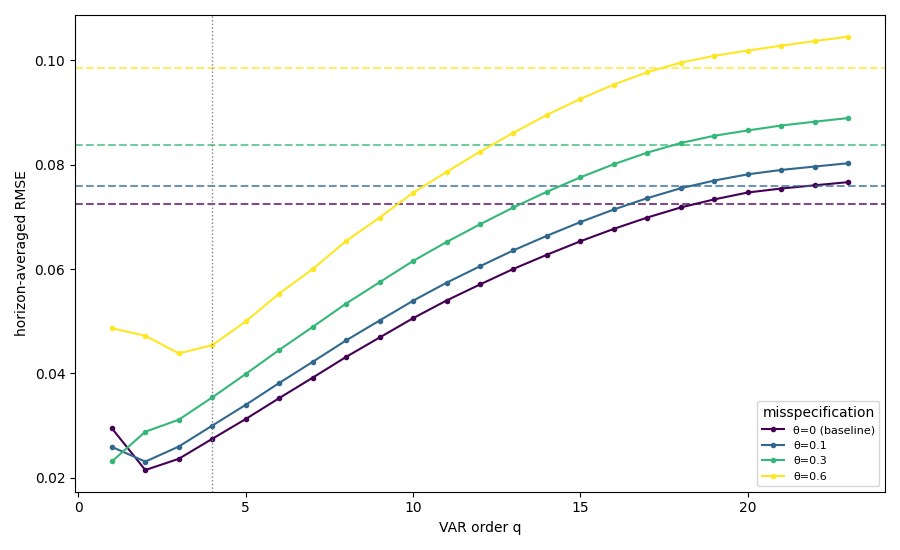
\includegraphics[width=\textwidth]{DYN_MISSPEC_COMPLEXITY_FRONTIER_rho=0.7_T=250.png}
            \caption{Complexity Frontier $\rho = 0.7$}
        \end{minipage}
        \hfill
        \begin{minipage}{0.59\textwidth}
            \centering
            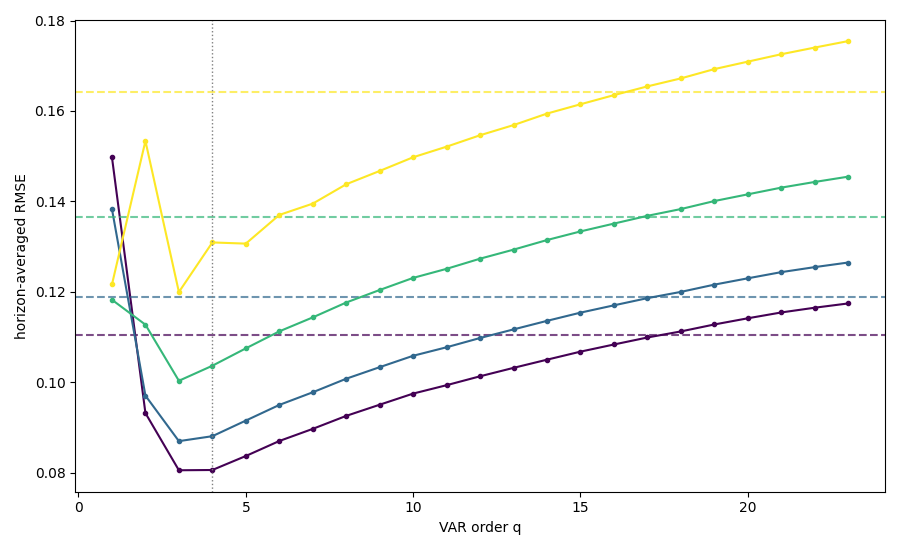
\includegraphics[width=\textwidth]{DYN_MISSPEC_COMPLEXITY_FRONTIER_rho=0.95_T=250.png}
            \caption{Complexity Frontier $\rho = 0.95$}
        \end{minipage}
    \end{figure}
\end{frame}

%--------------------------------------------------------------

\begin{frame}{Bias - Correct vs. Misspecification - $\tau = 0.6$}
    \setcounter{figure}{3}
    \begin{figure}
        \centering
        \begin{minipage}{0.39\textwidth}
            \centering
            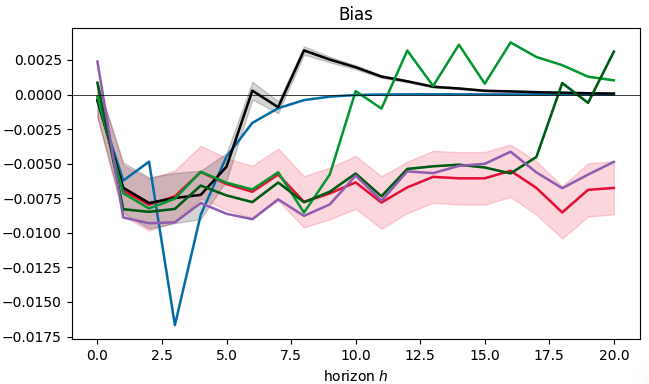
\includegraphics[width=\textwidth]{BASE_BIAS_0.5.png}
            \caption{Baseline at $\rho = 0.5$}          
        \end{minipage}
        \hfill
        \setcounter{figure}{12}                         
        \begin{minipage}{0.59\textwidth}
            \centering
            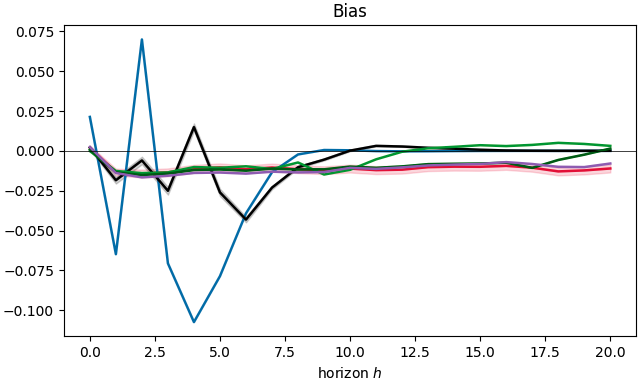
\includegraphics[width=\textwidth]{DYN_BIAS_0.5.png}
            \caption{Dyn. Misspecification at $\tau = 0.6$}  % → Figure 13
        \end{minipage}
    \end{figure}
\end{frame}

% \begin{frame}{Bias - Correct vs. Misspecification - $\rho = 0.95$}
%     \setcounter{figure}{5}
%     \begin{figure}
%         \centering
%         \begin{minipage}{0.39\textwidth}
%             \centering
%             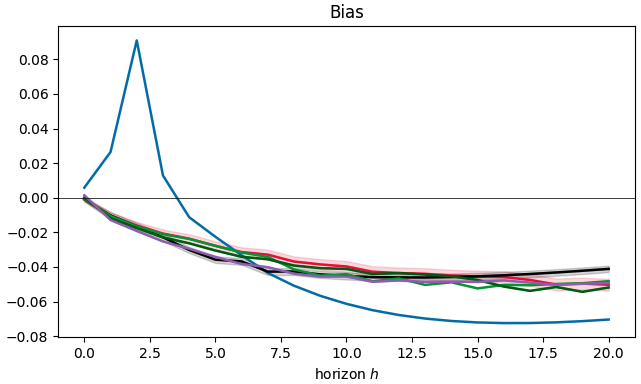
\includegraphics[width=\textwidth]{BASE_BIAS_0.95.png}
%             \caption{Baseline at $\rho = 0.95$}          % this needs correction if included
%         \end{minipage}
%         \hfill
%         \setcounter{figure}{13}                         % this needs correction if included
%         \begin{minipage}{0.59\textwidth}
%             \centering
%             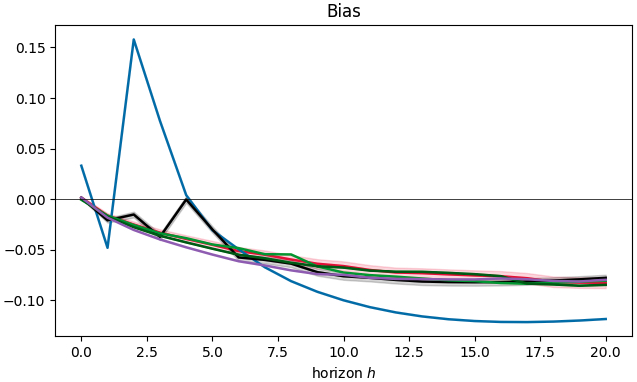
\includegraphics[width=\textwidth]{DYN_BIAS_0.95.png}
%             \caption{Dyn. Misspecification at $\rho = 0.95$ and $\tau = 0.6$}  % → Figure 13
%         \end{minipage}
%     \end{figure}
% \end{frame}

%--------------------------------------------------------------

\begin{frame}{Variance - Correct vs. Misspecification - $\tau= 0.6$}
    \setcounter{figure}{5}
    \begin{figure}
        \centering
        \begin{minipage}{0.39\textwidth}
            \centering
            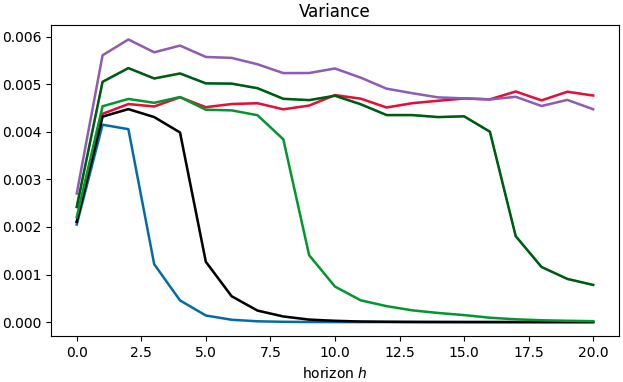
\includegraphics[width=\textwidth]{BASE_VAR_0.5.png}
            \caption{Baseline at $\rho = 0.5$}          
        \end{minipage}
        \hfill
        \setcounter{figure}{13}                         
        \begin{minipage}{0.59\textwidth}
            \centering
            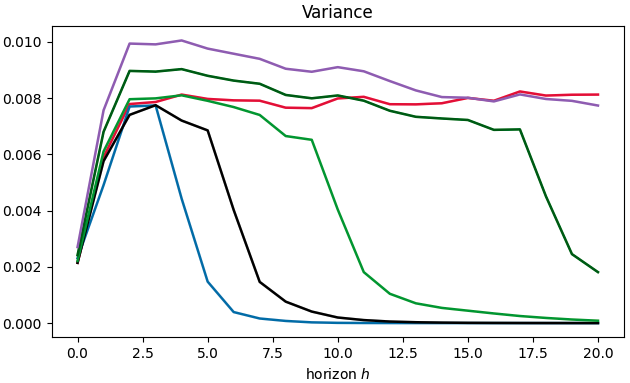
\includegraphics[width=\textwidth]{DYN_VAR_0.5.png}
            \caption{Dyn. Misspecification at $\tau = 0.6$}  % → Figure 13
        \end{minipage}
    \end{figure}
\end{frame}

% \begin{frame}{Variance - Correct vs. Misspecification - $\rho = 0.95$}
%     \setcounter{figure}{5}
%     \begin{figure}
%         \centering
%         \begin{minipage}{0.39\textwidth}
%             \centering
%             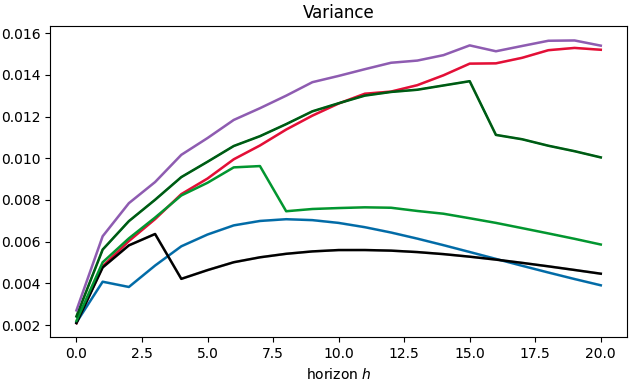
\includegraphics[width=\textwidth]{BASE_VAR_0.95.png}
%             \caption{Baseline at $\rho = 0.95$}          % this needs correction if included
%         \end{minipage}
%         \hfill
%         \setcounter{figure}{13}                         % this needs correction if included
%         \begin{minipage}{0.59\textwidth}
%             \centering
%             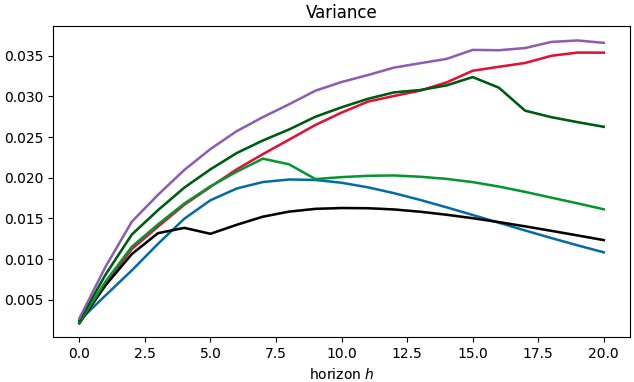
\includegraphics[width=\textwidth]{DYN_VAR_0.95.png}
%             \caption{Dyn. Misspecification at $\rho = 0.95$ and $\tau = 0.6$}  % → Figure 13
%         \end{minipage}
%     \end{figure}
% \end{frame}

%--------------------------------------------------------------

\begin{frame}{Coverage - Correct vs. Misspecification - $\tau = 0.6$}
    \setcounter{figure}{7}
    \begin{figure}
        \centering
        \begin{minipage}{0.39\textwidth}
            \centering
            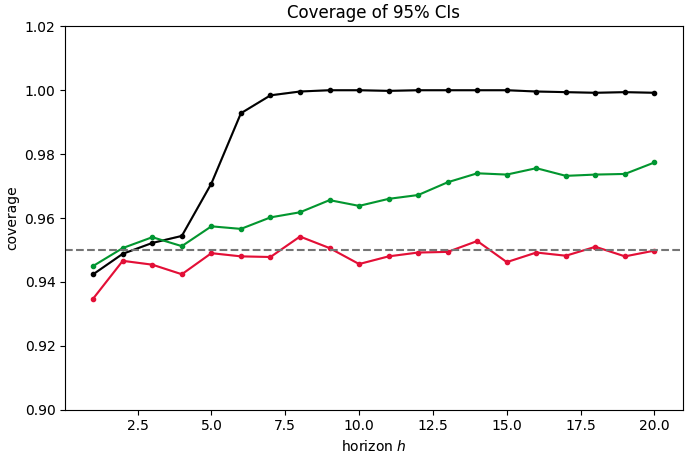
\includegraphics[width=\textwidth]{BASE_CI_0.5.png}
            \caption{Baseline at $\rho = 0.5$}          
        \end{minipage}
        \hfill
        \setcounter{figure}{14}                         
        \begin{minipage}{0.59\textwidth}
            \centering
            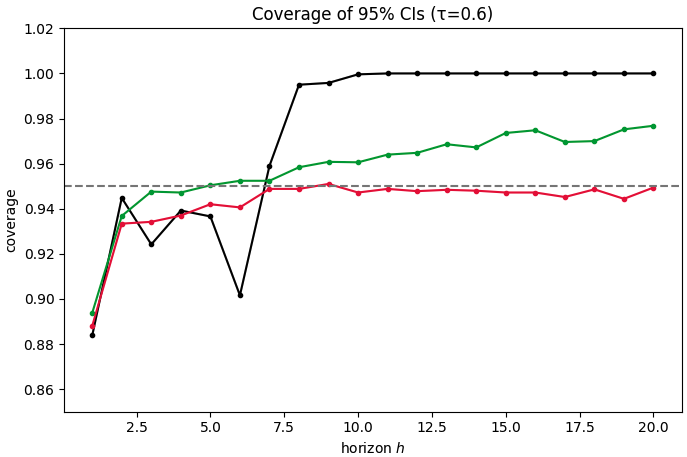
\includegraphics[width=\textwidth]{DYN_CI_0.5.png}
            \caption{Dyn. Misspecification at $\tau = 0.6$}  % → Figure 13
        \end{minipage}
    \end{figure}
\end{frame}

%------------------------------------------------
\begin{frame}{Introducing Functional Misspecification}

\begin{figure}
    \centering
    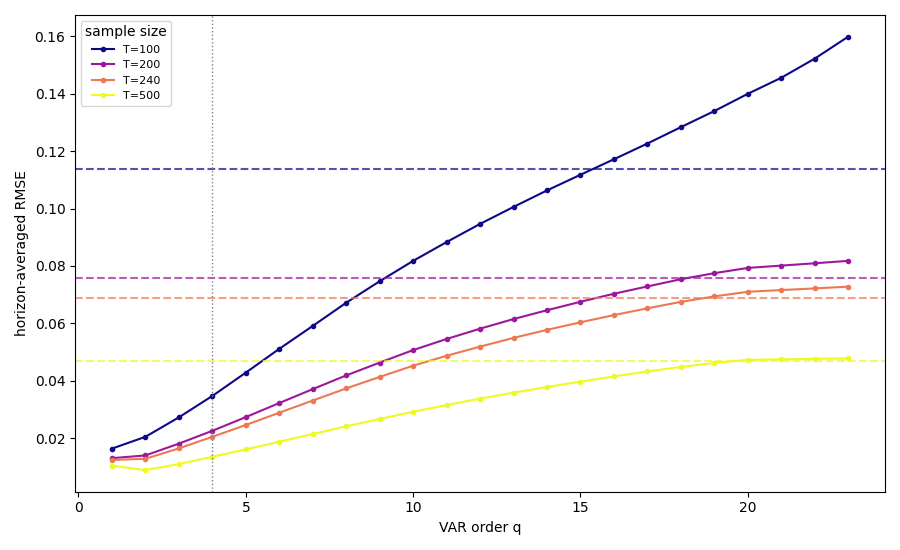
\includegraphics[width=0.7\linewidth]{BASE_COMPLEXITY_FRONTIER_rho=0.5.png}
    \vspace*{-0.2cm}
    \caption{}
\end{figure}
\end{frame}




\begin{frame}{Variance - Correct vs. Misspecification - $\rho = 0.5$}
    \setcounter{figure}{5}
    \begin{figure}
        \centering
        \begin{minipage}{0.39\textwidth}
            \centering
            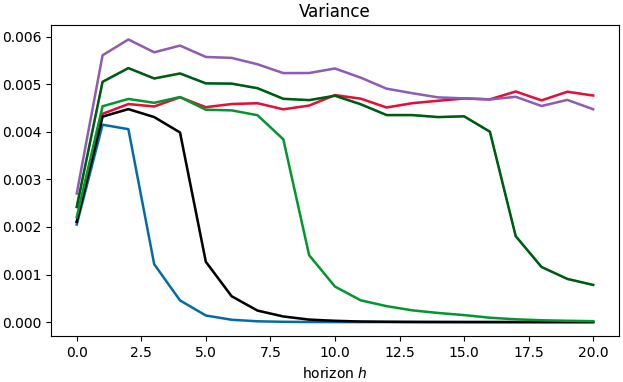
\includegraphics[width=\textwidth]{BASE_VAR_0.5.png}
            \caption{Baseline at $\rho = 0.5$}          
        \end{minipage}
        \hfill
        \setcounter{figure}{13}                         
        \begin{minipage}{0.59\textwidth}
            \centering
            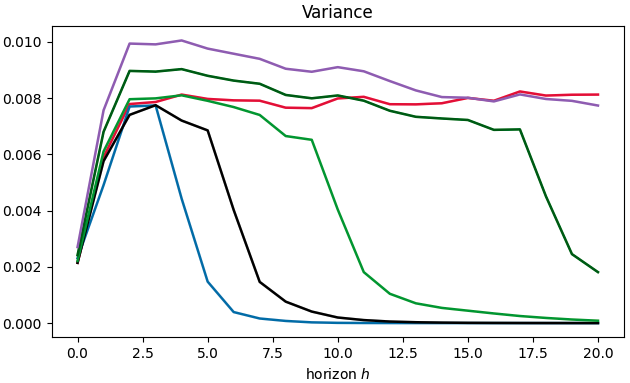
\includegraphics[width=\textwidth]{DYN_VAR_0.5.png}
            \caption{Dyn. Misspecification at $\gamma = 0.6$}  % → Figure 13
        \end{minipage}
    \end{figure}
\end{frame}






\begin{frame}{Coverage - Correct vs. Misspecification - $\rho = 0.5$}
    \setcounter{figure}{7}
    \begin{figure}
        \centering
        \begin{minipage}{0.39\textwidth}
            \centering
            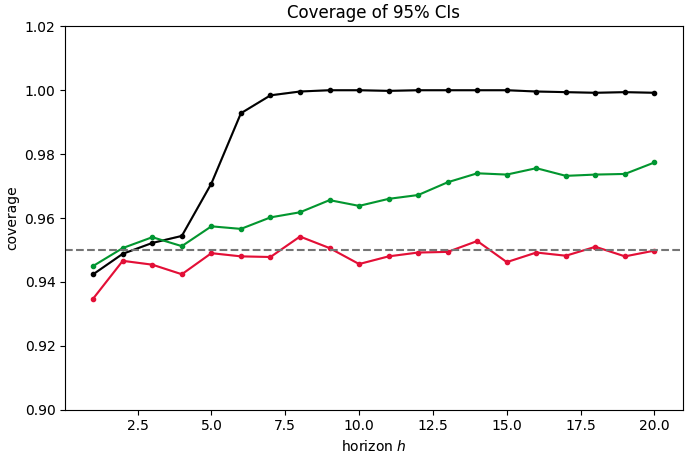
\includegraphics[width=\textwidth]{BASE_CI_0.5.png}
            \caption{Baseline}          
        \end{minipage}
        \hfill
        \setcounter{figure}{14}                         
        \begin{minipage}{0.59\textwidth}
            \centering
            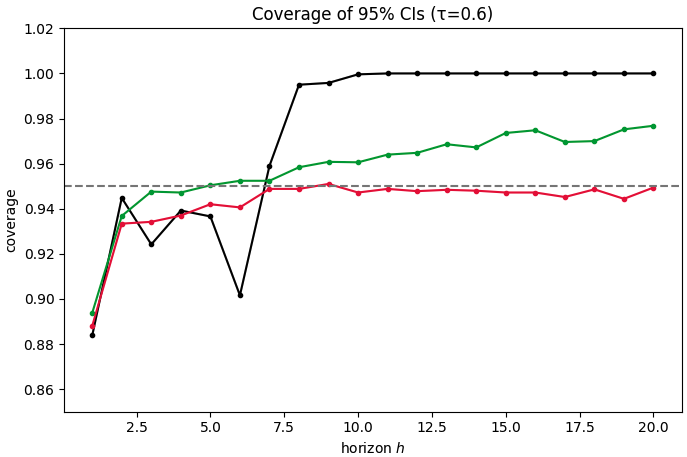
\includegraphics[width=\textwidth]{DYN_CI_0.5.png}
            \caption{Fct. Misspecification at $\gamma = 0.6$}  
        \end{minipage}
    \end{figure}
\end{frame}

%-----------------------------------------------------------------------------------

\section{Discussion}

\begin{frame}{Discussion of Results}

    \begin{itemize}
        \item LP(4) $\approx$ VAR(15)
        \item As $T$ decreases, LP(4) is equal to a less parsimonous VAR $\to$ relatively better
        \item As $\rho$ increases, LP(4) is equal to a less parsimonous VAR $\to$ relatively better
        \item \colorbox{orange!10}{As $\tau$ increases, LP(4) is equal to a less parsimonous VAR $\to$ relatively better}
        \item At equal lags, VAR(p) is preferable choice if applicable, except for coverage
        \item higher order VARs closes coverage gap, at cost of bias and variance
    \end{itemize}


    
\end{frame}

%-----------------------------------------------------------------------------------

\section{Conclusion}

\begin{frame}{Conclusion}
    \begin{enumerate}
        \item Ludwig identity largely consistent with MC findings
        \item 
        \item 
    \end{enumerate}


\end{frame}



\begin{frame}
Thank you for your Attention! Questions?


\end{frame}

% \begin{frame}[allowframebreaks]{Literaturverzeichnis}

%   \bibliography{references.bib}
%   \bibliographystyle{abbrv}

% \end{frame}


% \begin{frame}{Appendix}
% \appendix
% \begin{figure}
%     \centering
%     \includegraphics[width=0.35\linewidth]{}
%     \caption{}
% \end{figure}
% \end{frame}

%------------------------------------------------

\end{document}